% Q3V3: C-core, Aiding Dots, Symmetric — Physical winding diagram
% Both coils wound SAME DIRECTION on C-core (no gap)
% Does NOT show dot placements — that is Part (a) answer (P-STACK-31)
\documentclass[border=10pt]{standalone}
\usepackage{tikz}
\usepackage{amsmath}
\renewcommand{\familydefault}{\sfdefault}

\begin{document}
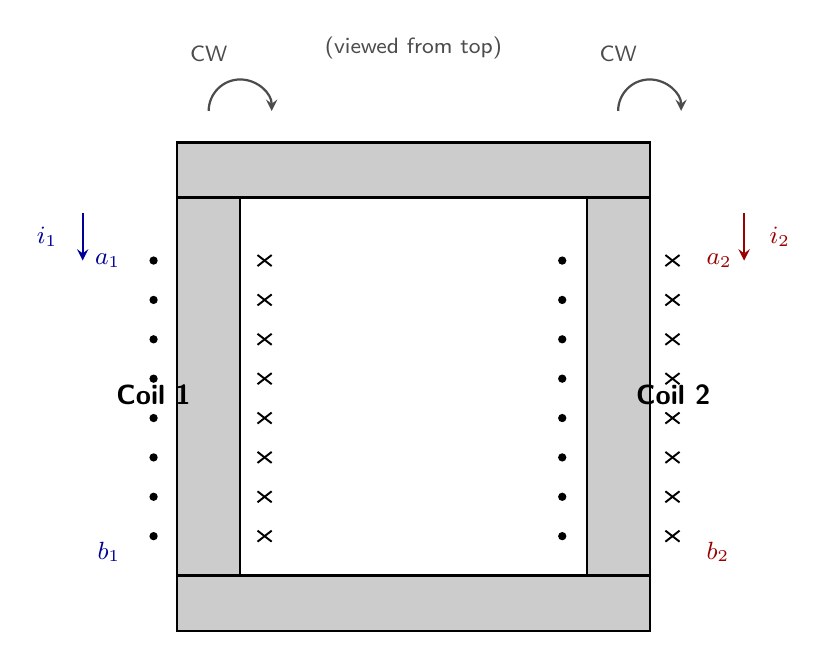
\begin{tikzpicture}[
    every node/.style={font=\sffamily},
    >=stealth,
]

% === C-core (no air gap) ===
\def\coreW{6}
\def\coreH{5.5}
\def\barH{0.7}
\def\limbW{0.8}

% Bottom yoke
\fill[gray!40, draw=black, line width=0.8pt]
    (0,0) rectangle (\coreW,\barH);
% Left limb
\fill[gray!40, draw=black, line width=0.8pt]
    (0,\barH) rectangle (\limbW,\coreH);
% Right limb
\fill[gray!40, draw=black, line width=0.8pt]
    ({\coreW-\limbW},\barH) rectangle (\coreW,\coreH);
% Top yoke (complete, no gap)
\fill[gray!40, draw=black, line width=0.8pt]
    (0,\coreH) rectangle (\coreW,{\coreH+\barH});

% === Coil 1 (left limb) — clockwise from top ===
% CW from top → dot on left, cross on right
\foreach \ycoil in {1.2, 1.7, 2.2, 2.7, 3.2, 3.7, 4.2, 4.7} {
    % Left: dot
    \fill ({-0.3},\ycoil) circle (1.5pt);
    % Right: cross
    \draw[line width=0.7pt] ({\limbW+0.22},{\ycoil-0.07}) -- ({\limbW+0.40},{\ycoil+0.07});
    \draw[line width=0.7pt] ({\limbW+0.22},{\ycoil+0.07}) -- ({\limbW+0.40},{\ycoil-0.07});
}

% Coil 1 labels (spaced to avoid overlap)
\node[font=\sffamily\bfseries] at ({-0.3}, 3.0) {Coil 1};
\node[left, font=\sffamily\small, text=blue!60!black] at (-0.6, 4.7) {$a_1$};
\node[left, font=\sffamily\small, text=blue!60!black] at (-0.6, 1.0) {$b_1$};
\draw[->, thick, blue!60!black] (-1.2, 5.3) -- (-1.2, 4.7);
\node[left, font=\sffamily\small, text=blue!60!black] at (-1.4, 5.0) {$i_1$};

% === Coil 2 (right limb) — SAME sense as Coil 1 ===
% Same CW from top → dot on left (inside face), cross on right (outside face)
\foreach \ycoil in {1.2, 1.7, 2.2, 2.7, 3.2, 3.7, 4.2, 4.7} {
    % Left (inner face): dot
    \pgfmathsetmacro{\leftX}{\coreW-\limbW-0.40}
    \fill ({\leftX+0.09},\ycoil) circle (1.5pt);
    % Right (outer face): cross
    \draw[line width=0.7pt] ({\coreW+0.20},{\ycoil-0.07}) -- ({\coreW+0.38},{\ycoil+0.07});
    \draw[line width=0.7pt] ({\coreW+0.20},{\ycoil+0.07}) -- ({\coreW+0.38},{\ycoil-0.07});
}

% Coil 2 labels (spaced to avoid overlap)
\node[font=\sffamily\bfseries] at ({\coreW+0.3}, 3.0) {Coil 2};
\node[right, font=\sffamily\small, text=red!60!black] at ({\coreW+0.6}, 4.7) {$a_2$};
\node[right, font=\sffamily\small, text=red!60!black] at ({\coreW+0.6}, 1.0) {$b_2$};
\draw[->, thick, red!60!black] ({\coreW+1.2}, 5.3) -- ({\coreW+1.2}, 4.7);
\node[right, font=\sffamily\small, text=red!60!black] at ({\coreW+1.4}, 5.0) {$i_2$};

% === Winding sense annotations ===
\draw[->, thick, gray!60!black] (0.4, 6.6) arc[start angle=180, end angle=0, radius=0.4];
\node[above, font=\sffamily\footnotesize, gray!60!black] at (0.4, 7.1) {CW};
\draw[->, thick, gray!60!black] ({\coreW-0.4}, 6.6) arc[start angle=180, end angle=0, radius=0.4];
\node[above, font=\sffamily\footnotesize, gray!60!black] at ({\coreW-0.4}, 7.1) {CW};
\node[font=\sffamily\footnotesize, gray!60!black] at ({0.5*\coreW}, 7.4) {(viewed from top)};

\end{tikzpicture}
\end{document}
